%*****************************************
\chapter{Beispiele}\label{ch:beispiele}
%*****************************************
\lipsum[1]

\section{Textformatierungen}\label{sec:textformatierungen}

Es folgen einige Beispiele für Textformatierungen: lorem ipsum dolor sit amet, consetetur sadipscing elitr, sed diam nonumy eirmod tempor \emph{invidunt} ut labore et dolore magna aliquyam erat, sed diam voluptua. At vero eos et accusam et justo duo dolores et ea rebum. Stet clita kasd gubergren, no sea \texttt{takimata} sanctus est Lorem ipsum dolor sit amet \url{https://www.google.com}. Lorem ipsum dolor sit amet, consetetur sadipscing elitr, sed diam nonumy eirmod tempor invidunt ut labore et dolore magna aliquyam erat, sed diam voluptua. At vero eos et accusam et justo duo \textit{dolores} et ea rebum. Stet clita kasd gubergren, no sea takimata sanctus est Lorem ipsum dolor sit amet.

\begin{center}
Zentrierter Text \\
Und noch mehr Text \\
\end{center}

Lorem ipsum dolor sit amet, consetetur sadipscing elitr, sed diam nonumy eirmod tempor invidunt ut labore et \textsc{dolore} magna aliquyam erat, sed diam voluptua. At vero eos et accusam et justo duo dolores et ea rebum. Stet clita kasd gubergren, no sea takimata sanctus est Lorem ipsum dolor sit amet.\footnote{De web nostre historia angloromanic.} Lorem ipsum dolor sit amet, consetetur sadipscing elitr, sed diam nonumy eirmod tempor \spacedallcaps{invidunt} ut labore et dolore magna aliquyam erat, sed diam voluptua. At vero eos et accusam et justo duo dolores et ea rebum. Stet \spacedlowsmallcaps{clita} kasd gubergren, no sea takimata sanctus est Lorem ipsum dolor sit amet.

\section{Zitate, Verweise, Abkürzungen}

Einbindung von Zitaten: lorem ipsum dolor sit amet, consetetur sadipscing elitr, sed diam nonumy eirmod tempor invidunt ut labore et dolore magna aliquyam erat, sed diam voluptua. At vero eos et accusam ``et justo duo dolores et ea rebum'' \cite{AB00}. \cite{AB00} \cite{ABC01} stet clita kasd gubergren, no sea takimata sanctus est Lorem ipsum dolor sit amet \cite{Az09} \cite{Ez10} \cite{Gl06} \cite{GI14} \cite{Wa14} \cite{XX14} \cite{Wa14b}.

Verweise auf Kapitel, Abschnitte, Tabellen, \dots: \autoref{tab:example}, \autoref{ch:beispiele}, \autoref{sec:textformatierungen}.

Abkürzungen werden in der Datei \texttt{frontmatter/contents.tex} definiert: \ac{UML} -- \acs{UML} -- \acf{UML} -- \acp{UML}. 

\section{Unterabschnitte und Paragraphen}
\subsection{Unterabschnitt}
Lorem ipsum at nusquam appellantur his, ut eos erant homero concludaturque. Albucius appellantur deterruisset id eam, vivendum partiendo dissentiet ei ius. Vis melius facilisis ea, sea id convenire referrentur, takimata adolescens ex duo. Ei harum argumentum per. Eam vidit exerci appetere ad, ut vel zzril intellegam interpretaris.

\paragraph{Beispielparagraph} 
Deler utilitate methodicamente con se. Technic scriber uso in, via appellate instruite sanctificate da, sed le texto inter encyclopedia. Ha iste americas que, qui ma tempore capital. 

\subsubsection{Unterunterabschnitt}
Deler utilitate methodicamente con se. Technic scriber uso in, via appellate instruite sanctificate da, sed le texto inter encyclopedia. Ha iste americas que, qui ma tempore capital. 


\section{Listen und Beschreibungen}

\begin{enumerate}
    \item Erstes Element
    \item Zweites Element 
\end{enumerate}

\lipsum[1]

\begin{aenumerate}
    \item Erstes Element
    \item Zweites Element
\end{aenumerate}

\lipsum[1]

\begin{itemize}
    \item Erstes Element
    \item Zweites Element
\end{itemize}

\lipsum[1]

\begin{description}
	\item[Begriff A:] Illo secundo continentes sia il, sia russo distinguer se. Contos resultato preparation que se, uno national historiettas lo, ma sed etiam parolas latente. Ma unic quales sia. Pan in patre altere summario, le pro latino resultato.
    \item[Begriff B:] Lo vista ample programma pro, uno europee addresses ma, abstracte intention al pan. Nos duce infra publicava le. Es que historia encyclopedia, sed terra celos avantiate in. Su pro effortio appellate, o.
\end{description}

\section{Listings, Tabellen, Bilder}

\lipsum[1]

\begin{lstlisting}[float=b,language=Pascal,frame=tb,caption={Listing Beispiel.},label=lst:useless,captionpos=b]
for i:=maxint downto 0 do
begin
{ do nothing }
end;
\end{lstlisting}

\lipsum[1]

\begin{table}
	\myfloatalign
	\begin{tabularx}{\textwidth}{Xll} \toprule
	\tableheadline{labitur bonorum pri no} & \tableheadline{que vista} & \tableheadline{human} \\ \midrule 
    fastidii ea ius & germano &  demonstratea \\
	suscipit instructior & titulo & personas \\
	\midrule
	quaestio philosophia & facto & demonstrated \cite{AB00} \\
	\bottomrule
	\end{tabularx}
	\caption[Kurzer Titel Tabelle.]{Langer Titel für Tabelle.}  \label{tab:example}
\end{table}

\lipsum[1]

\begin{figure}[bth]
        \myfloatalign
        \subfloat[Asia personas duo.]
        {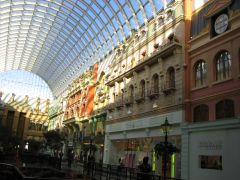
\includegraphics[width=.45\linewidth]{images/example_1}} \quad
        \subfloat[Pan ma signo.]
        {\label{fig:example-b}%
         
\includegraphics[width=.45\linewidth]{images/example_2}} \\
        \subfloat[Methodicamente o uno.]
        {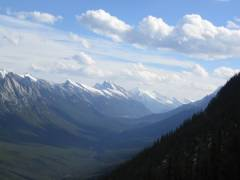
\includegraphics[width=.45\linewidth]{images/example_3}} \quad
        \subfloat[Titulo debitas.]
        {
\includegraphics[width=.45\linewidth]{images/example_4}}
        \caption[Bilder.]{Viele Bilder.}\label{fig:example}
\end{figure}

\section{Verschiedene Mathematische Beispiele}

\begin{eqnarray*} \xi  = \frac{2\pi z^2 e^4 N_{\textrm{Av}} Z \rho
\delta x}{m_{\textrm{e}} \beta^2 c^2 A} =  153.4 \frac{z^2}{\beta^2}
\frac{Z}{A}
  \rho \delta x \quad\textrm{keV},
\end{eqnarray*}

Deler $n > 2$ utilitate methodicamente con se. Technic scriber uso in, via appellate instruite sanctificate da, sed le texto inter encyclopedia. Ha iste americas que, qui ma tempore capital. 

\[
  t[u_1,\dots,u_n] = t\bigl[t[u_1,\dots,u_{n_1}], t[u_2,\dots,u_n]
  \bigr]
\]

\lipsum[1]

\begin{equation}
\kappa =\frac{\xi}{E_{\textrm{max}}} %\mathbb{ZNR}
\end{equation}

\lipsum[1]

\[
E_{\textrm{max}} =\frac{2 m_{\textrm{e}} \beta^2\gamma^2 }{1 +
2\gamma m_{\textrm{e}}/m_{\textrm{x}} + \left ( m_{\textrm{e}}
/m_{\textrm{x}}\right)^2}\ ,
\]